\section{Linear Time Invariant Systems}

There is a branch of controls called Linear Time Invariant (LTI)
Systems that is often taught at the undergraduate level. Although
almost every system encountered in standard applications whether
aerospace or not are non-linear, it is still beneficial and more
simple to learn about control system dynamics when the system
parameters are constant and linear. 

\subsection{Linearization of Non-Linear Systems}

Standard nonlinear dynamics can be placed into standard
nonlinear affine form as shown below after much simplification of
terms
\begin{equation}
  \dot{\vec{x}} = \vec{f}(\vec{x}) + \vec{g}(\vec{x})\vec{u}
\end{equation}
where $\vec{u}$ is the control input which could be the forces and
moments from reaction wheels or thrusters for a spacecraft or lift and drag for an airplane. The vectors $f$ and $g$ represent the systems dynamics which is dependent on the system itself. Note that if the dynamics cannot be put into affine form, the system is highly nonlinear and the control system designed for that would require more sophisticated analysis like Lyapunov design or sliding mode control. That will be discussed in a later section. For the affine form however, the equation can be
linearized to give the equation below. 
\begin{equation}\label{e:linearize}
  \Delta \dot{\vec{x}} = {\bf A}\Delta {\vec{x}} + {\bf B}\Delta \vec{u}
\end{equation}
where $\Delta \vec{x} = \vec{x} - \vec{x}_e$ and $\vec{x}_e$ is an
equilibrium point. In this formulation ${\bf A} = \partial \vec{f}/\partial \vec{x}$. and 
${\bf B} = \partial \vec{g}/\partial \vec{x}$ which are partial derivatives of the state matrices. Note that an equilibrium point is a point where the system is at rest and not changing. Mathematically this means that $\dot{x}_e = 0$. When linearizing a system it is important to choose an equilibrium point that is relevant to the system. For example, for an aircraft the equilibrium point could be straight and level flight at a constant velocity. For a spacecraft it could be a circular orbit at a constant altitude. The linearized equations of motion are only valid for small perturbations around the equilibrium point. If the system deviates too far from the equilibrium point, the linearized equations may no longer accurately represent the system's dynamics.

\subsection{General Formulation of Differential Equations}

The linear systems of equations derived above are in state space form. That is the vector $\vec{x}$ contains all the states of the system. However, it is often easier to understand the dynamics of a system when it is in the form of a single differential equation with all states and derivatives shown in the same equation. Practical examples also help the undergraduate controls engineer as math with practical context is the best way to learn in my humble opinion. The sections below will discuss first and second order systems which are the most common types of systems encountered in engineering applications. Note that higher order systems can be reduced to first and second order systems by using techniques such as root locus or pole placement since higher order systems typically have high frequency dynamics that can be ignored for control purposes. For the most part, first and second order systems are all that is needed to understand the basics of control systems and represent the majority of systems encountered in practice.

\subsubsection{First Order Systems}

A first order system undergoing free motion will have dynamics that look like this
\begin{equation} \label{e:first_order}
\dot{q} + \sigma q = \sigma f
\end{equation}
\noindent where q is a generalized coordinate, $\sigma$ is the inverse of the time constant $\tau$, and f is the forcing function. Examples of these types of systems in include thermistors, servos, and velocity equations for system dynamics. 

\subsubsection{Second Order Systems}

A second order system undergoing free motion will have dynamics that look like this
\begin{equation}\label{e:second_order}
\ddot{q} + 2\zeta \omega_n \dot{q} + {\omega_n}^2 q = {\omega_n}^2 f
\end{equation}
where $q$ is a generalized coordinate, $\sigma$ is the inverse of the time constant $\tau$, f is the forcing function, $\omega_n$ is the natural frequency of the system and $\zeta$ is the damping ratio. Examples of these types of systems include mass, spring dampers in linear translation as well as torsional systems and penduluums. Anything that oscillates will exhibit this behavior. 

\subsection{Equation of Motion Formulation for Practical Systems}

The sections below will discuss practical examples of first and second order systems. Many of these examples are classic examples found in many dynamics and controls textbooks and ones that I typically teach budding control systems aerospace/mechanical engineers. Each one offers a slightly different set of dynamics and challenges that will help the undergraduate controls engineer understand the concepts of linear systems as well as how to control them and also determine stability. 

\subsubsection{Position and Velocity of a Car}

Consider a car moving in one dimension. The primary forces acting on the car are the driving force from the tires, $F$, and a linear viscous drag force, $D = -cv$, where $c$ is the viscous drag coefficient, $x$ is the position of the car and $v$ is the velocity of the car.
\begin{figure}[H]
    \centering
    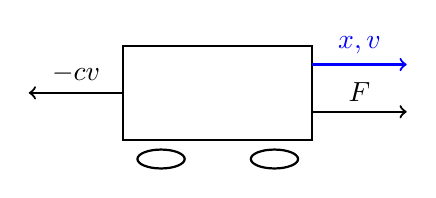
\begin{tikzpicture}[scale=1.2]
        % Draw the car as a rectangle
        \draw[thick] (0,0) rectangle (2,1);
        % Wheels
        \draw[thick] (0.4,-0.2) ellipse (0.25 and 0.1);
        \draw[thick] (1.6,-0.2) ellipse (0.25 and 0.1);
        % Forces
        \draw[->,thick] (2,0.3) -- ++(1,0) node[midway, above] {$F$};
        \draw[->,thick] (0,0.5) -- ++(-1,0) node[midway, above] {$-cv$};
        % Velocity arrow
        \draw[->,thick,blue] (2.0,0.8) -- ++(1,0.0) node[midway, above] {$x,v$};
    \end{tikzpicture}
    \caption{Free body diagram of a car}
    \label{f:car_fbd}
\end{figure}
\noindent Applying Newton's second law, the sum of forces is equal to mass times acceleration:
\begin{equation}
  m\dot{v} = F - cv
\end{equation}
where $m$ is the mass of the car, $F$ is the force generated by the tires, and $-cv$ is the linear drag. In this case to make the system first order we simply leave acceleration as $\dot{v}$ instead of $\ddot{x}$ where x would be the position of the vehicle. Rearranging, we obtain the standard first-order linear differential equation:
\begin{equation}
  \dot{v} + \frac{c}{m}v = \frac{F}{m}
\end{equation}
This equation describes the velocity dynamics of the car under a linear drag assumption. In this case $\sigma = c/m$ and $F = cf$. With these substitutions you arrive at the same equation as \ref{e:first_order}. Note that if $v$ is replaced with $\dot{x}$ and $\dot{v}$ is replaced with $\ddot{x}$ the equation describes the position of car and is second order as shown below.
\begin{equation}
    \ddot{x} + \frac{c}{m}\dot{x} = \frac{F}{m}
\end{equation}
This is another general second order system where the natural frequency ${\omega_n}^2=0$. Using the same substitions as above the general formulation is 
\begin{equation}
    \ddot{q} + \sigma \dot{q} = \sigma f
\end{equation}
where $x$ is replaced by $q$. The result is similar to the first order system but still slightly different. given the absence of the constant term. It will be shown later that this system is marginally stable and that the difference between the first and second order transfer function is simply a factor of s given the difference from velocity to position.

\subsubsection{Position of a Mass Spring Damper}

A mass-spring-damper system is a classic example of a second-order system. The system consists of a mass $m$ attached to a spring with spring constant $k$ and a damper with damping coefficient $c$. The mass is free to move along a single axis $x$, and the system is subject to an external force $f$ as shown in Figure \ref{f:msd}.

\begin{figure}[H]
    \centering
    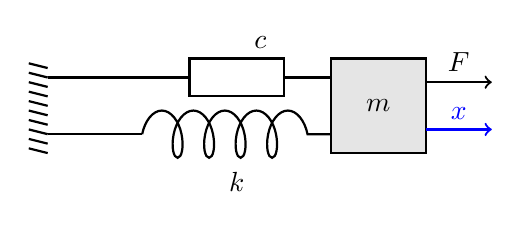
\begin{tikzpicture}[scale=1.2]
        % Draw the wall
        \draw[thick] (-1,.2) -- (0,0.2);
        \draw[thick] (-1,0.8) -- (0,0.8);
        \foreach \y in {0,0.1,...,1.0}
            \draw[thick] (-1,\y) -- (-1.2,\y+0.05);

        % Draw the spring
        \draw[thick,decorate,decoration={coil,aspect=0.5,segment length=4mm,amplitude=3mm}] (0,0.2) -- (2,0.2);

        % Draw the damper
        \draw[thick] (0,0.8) -- (0.5,0.8);
        \draw[thick] (0.5,1.0) rectangle (1.5,0.6);
        \draw[thick] (1.5,0.8) -- (2.0,0.8);

        % Draw the mass
        \draw[thick,fill=gray!20] (2,0) rectangle (3,1.0);

        % Labels
        \node at (2.5,0.5) {$m$};
        \node[above] at (1.25,1.0) {$c$};
        \node[below] at (1,-0.1) {$k$};
        \draw[->,thick,blue] (3.0,0.25) -- ++(0.7,0) node[midway, above] {$x$};
        \draw[->,thick] (3.0,0.75) -- ++(0.7,0) node[midway, above] {$F$};
    \end{tikzpicture}
    \caption{Mass-spring-damper system}
    \label{f:msd}
\end{figure}

Consider the mass-spring-damper system depicted above. The spring exerts a restoring force $-kx$ that is always directed opposite to the displacement $x$ of the mass from equilibrium, while the damper exerts a resistive force $-c\dot{x}$ proportional and opposite to the velocity $\dot{x}$. The external force $F(t)$ acts in the direction of motion. According to Newton's second law, the sum of these forces acting on the mass equals the mass times its acceleration, leading to the equation 
\begin{equation}
m\ddot{x} = F - c\dot{x} - kx 
\end{equation}
Rearranging terms, we obtain the standard form of the equation of motion for the mass-spring-damper system.
\begin{equation}
\ddot{x} + \frac{c}{m}\dot{x} + \frac{k}{m}x = \frac{F}{m}
\end{equation}
This second-order linear differential equation fully describes the dynamic response of the system to any external force $F$. Looking at equation \ref{e:second_order} we can see that $\omega_n = \sqrt{k/m}$ and $\zeta = c/(2\sqrt{mk})$. Furthermore, if we let $F = kf$ we arrive at the same equation as \ref{e:second_order}.

\subsubsection{Attitude Dynamics of a Satellite or Quadcopter}

For a satellite undergoing free 1-D rotational motion the dynamics are quite interesting from a controls perspective given the somewhat marginal stability of the satellite. The same can be said for a quadcopter undergoing slow rotational motion. In this case, it is assumed that the spacecraft or quadcopter rotates through the angle $\theta$ about its center of mass. The spacecraft/quadcopter has a moment of inertia $J$ and is subject to an external torque $\tau$ as shown in Figure \ref{f:satellite}. In this case ,the torque is created by reaction control thrusters or propellors with a force $F$ at a distance $d$ from the center of mass. Note that in the case of the satellite there are 4 thrusters but only 2 operate at a time. If the top right and bottom left thrusters fire the torque is negative and if the top left and bottom right thrusters fire the torque is positive. In this case we let $F_1=F_2=F_3=F_4=F$. If $F>0$ it means it is a positive torque and $F_1=F_4$ are non-zero while $F_2=F_3=0$. If $F<0$ the torque is negative and $F_1=F_4=0$ while $F_2=F_3$ are non-zero. For a quadcopter the 4 propellors are offset by a nominal thrust to keep the quadcopter aloft. Furthermore, since the quadcopter is symmetric about the rotational axis it can be assumed that the quadcopter only has 2 propellors $F_3$ and $F_4$. The torque is created by increasing the thrust on one side and decreasing it on the other side. In this case $F_3=F_H+\Delta F$, $F_4=F_H-\Delta F$ where $F_H$ is the thrust required for hovering. Adding the effect of $F_3$ and $F_4$ yields $2\Delta F$ which can just be replaced with $2F$ and the formulation can continue. 
\begin{figure}[H]
    \centering
    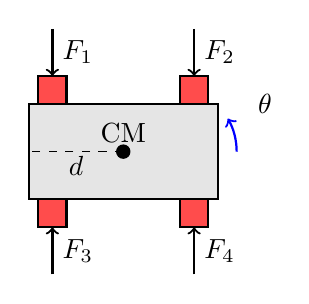
\begin{tikzpicture}[scale=1.2]
        % Draw the satellite body
        \draw[thick,fill=gray!20] (0,0) rectangle (2,1);
        
        % Draw the thrusters
        \draw[thick,fill=red!70] (0.1,1.0) rectangle (0.4,1.3);
        \draw[thick,fill=red!70] (1.6,1.0) rectangle (1.9,1.3);
        \draw[thick,fill=red!70] (0.1,-0.3) rectangle (0.4,0);
        \draw[thick,fill=red!70] (1.6,-0.3) rectangle (1.9,0);
        
        % Draw the forces from thrusters
        \draw[->,thick] (0.25,1.8) -- ++(0,-0.5) node[midway, right] {$F_1$};
        \draw[->,thick] (1.75,1.8) -- ++(0,-0.5) node[midway, right] {$F_2$};
        \draw[->,thick] (0.25,-0.8) -- ++(0,0.5) node[midway, right] {$F_3$};
        \draw[->,thick] (1.75,-0.8) -- ++(0,0.5) node[midway, right] {$F_4$};
        
        % Draw the center of mass
        \filldraw[black] (1,0.5) circle (2pt);
        \node at (1,0.7) {CM};
        
        % Draw the angle theta
        \draw[->,thick,blue] (2.2,0.5) arc[start angle=0,end angle=30,radius=0.7];
        \node at (2.5,1) {$\theta$};
        
        % Draw the distance d
        \draw[dashed] (1,0.5) -- (0,0.5);
        \node at (0.5,0.35) {$d$};
    \end{tikzpicture}
    \caption{Satellite with reaction control thrusters}\label{f:satellite}
\end{figure}

The equation of motion for the satellite can be derived from Newton's second law for rotational motion, which states that the sum of torques acting on a body equals the moment of inertia times its angular acceleration as derived in Section \ref{s:rotational_motion}. The full equation is repeated here for clarity.
\begin{equation}
\vec{M}_C = \dot{{\bf I}}\vec{\omega}_{B/I} + {\bf I}_C\frac{{}^Bd (\vec{\omega}_{B/I})}{dt} + {\bf
  S}(\vec{\omega}_{B/I}){\bf I}_C\vec{\omega}_{B/I}
\end{equation}
In this section however the inertia is constant, thus the entire first term goes to zero, and since the motion of the satellite is planar the third term is also zero. Thus, the equation reduces to
\begin{equation}
\vec{M}_C = {\bf I}_C\frac{{}^Bd (\vec{\omega}_{B/I})}{dt} = J \vec{\alpha}_{B/I} = J\ddot{\theta}
\end{equation}
where $\vec{\alpha}_{B/I}$ is the angular acceleration of the satellite. The torque generated by the thrusters is given as $\vec{M}_C = \tau = 2Fd$. The multiplication by 2 is due to 2 thrusters firing at a time or in the case of the quadcopter it is due to the symmetry of the rotation axis as explained above. The final equations of motion for the satellite/quadcopter are then given as
\begin{equation}
\ddot{\theta} = \frac{2Fd}{J}
\end{equation}
This is a classic second order system where $\omega_n = 0$ and $\zeta = 0$. This means that the system is marginally stable and will not return to equilibrium after a disturbance. Stability will be discussed in a later section. Letting $F=f\frac{J}{2d}$ results in $\ddot{\theta}=f$ which is almost the same equation as equation \ref{e:second_order} but where the natural frequency and damping ratio are both zero. 

\subsubsection{Pitch Dynamics of an Aircraft}

For an aircraft we assume that the aircraft is symmetric about the longitudinal axis and that the aircraft is only pitching about its center of mass. The pitch dynamics of an aircraft are similar to a spring mass damper since there is a constant restoring moment given by $C_{m\alpha}$ due to the aerodynamic forces acting on the aircraft as well as a damping term $C_{mq}$ also created by aerodynamic forces. Using the aerodynamic equations given in Equation \ref{e:LMN}, the pitch dynamics of an aircraft are given as
\begin{equation}
    I_{yy}\ddot{\theta} = \vec{M_C} = \frac{1}{2}\rho V^2 S \bar{c} (C_{m\alpha}\theta + C_{mq}\frac{\bar{c}}{2V}\dot{\theta} + C_{m\delta_e}\delta_e)
\end{equation}
Note that in this case we assume that $\theta=\alpha$ the angle of attack which is not necessarily true but for quick motion about the pitch axis this can be assumed to be true. Again the moment of inertia is $I_{yy}$ and the pitch angle is $\theta$. The aerodynamic force is given by the dynamic pressure $q = (1/2)\rho V^2$ where $\rho$ is the density of air, $V$ is the velocity of the aircraft (assumed to be constant for pure pitching), $S$ is the reference area and $\bar{c}$ is the mean aerodynamic chord. The moment coefficients are $C_{m\alpha}$ which is the restoring moment coefficient, $C_{mq}$ which is the damping moment coefficient and $C_{m\delta_e}$ which is the control moment coefficient due to elevator deflection $\delta_e$. Rearranging the equation into standard form yields
\begin{equation}
    \ddot{\theta} + \left(-\frac{\rho V^2 S \bar{c}^2 C_{mq}}{4I_{yy} V}\right)\dot{\theta} + \left(-\frac{\rho V^2 S \bar{c} C_{m\alpha}}{2I_{yy}}\right)\theta = -\frac{\rho V^2 S \bar{c} C_{m\delta_e}}{2I_{yy}}\delta_e
\end{equation}
which is in the standard form of second order systems with a natural frequency and damping ratio given as 
\begin{equation}
    {\omega_n}^2 = -\frac{\rho V^2 S \bar{c} C_{m\alpha}}{2I_{yy}}, \quad \zeta = -\frac{\rho V^2 S \bar{c}^2 C_{mq}}{8I_{yy} V {\omega_n}}
\end{equation}
Note that $C_{m\alpha}$ and $C_{mq}$ are typically negative which makes both $\omega_n$ and $\zeta$ positive. However, in the case of the F-16 $C_{m\alpha}$ is actually negative. In this case the natural frequency squared becomes negative and the solution quite different. In The control term is the elevator deflection $\delta_e$ which means performing the final substitution below
\begin{equation}
    \delta_e = f \frac{C_{m\alpha}}{C_{m\delta_e}}
\end{equation}
results in the same equation as equation \ref{e:second_order} provided you subsitute $\theta$ with the generalized q coordinate. 

\subsubsection{Pitch Dynamics of a Rocket}

The pitch dynamic of a rocket are interesting in that the system is also marginally stable much like the satellite/quadcopter systems explained above. The difference of course is that the system is in the presence of the atmosphere and thus the aerodynamic forces create a damping effect which is proportional to the square of the velocity. This damping term is also nonlinear. However, in order to make the system linear it is assumed that the velocity is constant. For the sake of clarity the full equations of motion will be shown and then simplified to attain a simple linear form. First, the free body diagram of the rocket is shown in the Figure below.
\begin{figure}[H]
    \centering
    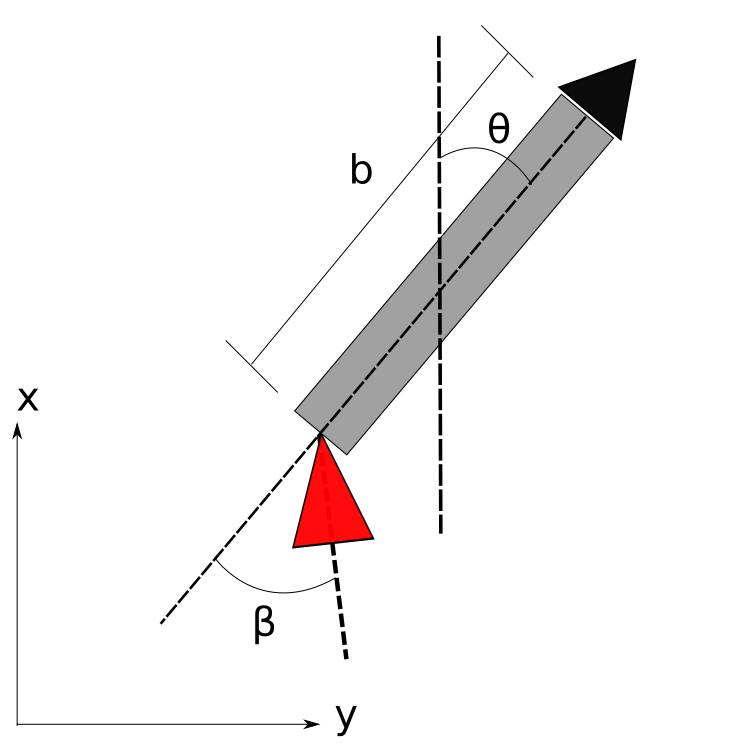
\includegraphics[width=0.5\textwidth]{Figures/Rocket.png}
    \caption{Rocket Pitch Dynamics Free Body Diagram}
\end{figure}
Here thrust acts at an angle $\beta$ with respect to the centerline of the rocket with a thrust equal to $T$. The length of the rocket is $b$ and thus the moment arm of the thrust vector is $b/2$. The aerodynamic force $D$ acts at the center of pressure which is a distance $c$ from the center of mass. It is assumed that the rocket is constantly traveling upwards and thus the Drag force $D$ is always pointed down at a distance of $a$ from the center of mass. The moment of inertia of the rocket is $J$ and the pitch angle is $\theta$. The equations of motion are similar to the quadcopter/satellite system undergoing 1-D rotational motion with a few subtle differences. 
\begin{equation}
    J\ddot{\theta} = \vec{M_C} = -D a \sin{\theta} + \frac{Tb}{2} \sin(\beta)
\end{equation}
First you'll see that the aerodynamic force which is restoring is nonlinear due to the $\sin{\theta}$ term. Furthermore, the thrust force $T$ acts through the angle $\beta$ leading to a problem where the thrust force $T$ could change in addition to the angle $\beta$. Two control terms would represent a multi-input system which requires the use of optimization to determine the best course of action. Since the focus of this chapter is on Single-Input-Single-Ouput (SISO) systems, the force $T$ will be represented as a constant. Thus, the control term for this system will actually be the angle $\beta$. However, note that the control term is also nonlinear. Both $sin()$ terms can be linearized for small angles such that $\sin{\theta} \approx \theta$ and $\sin{\beta} \approx \beta$. Note that $\theta=0$ is the equilibrium position in this case. The equation of motion then becomes
\begin{equation}
    J\ddot{\theta} + D a \theta = T \frac{b}{2} \beta
\end{equation}
Which is linear...almost. The second issue in this equation is that the aerodynamic force is a function of velocity squared. The drag force is given in Equations \ref{e:rocket_q} and \ref{e:aeroF}. As stated above it is assumed that the velocity is constant and thus $D$ is constant as well. The final equation of motion for the rocket pitch dynamics is then given as
\begin{equation}
    \ddot{\theta} + \frac{\pi}{J8}\rho V^2 d^2 a \theta = \frac{Tb}{2J} \beta
\end{equation}
If $(\pi/(J8))\rho V^2 d^2 a = {\omega_n}^2$, $Tb/(2J) \beta = \kappa {\omega_n}^2 f$ and $\theta = q$, the equations of motion are identical to the general form of second order systems except that $\kappa$ is a gain applied to the forcing function.  
\begin{equation}
    \ddot{q} + {\omega_n}^2 q = \kappa {\omega_n}^2 f
\end{equation}
In addition, it is clear that the damping ratio $\zeta$ is zero. 

\subsubsection{Pitch Dynamics of a Pendulum}

The dynamics of a pendulum are interesting for two reasons. First, the system is non-linear in the angle $\theta$ and the system has an infinite number of equilibrium points. Half of the equilibrium points are also unstable. For the sake of this problem though we will restrict the system to be between $-\pi$ and $\pi$ which means the system will only have 3 equilibrium points. The first is $\theta=0$ and the other two are $\theta=-\pi$ and $\theta=\pi$. Obviously the second two equilibrium points are the same. To formulate the dynamics we start with the figure below
\begin{figure}[H]
    \centering
    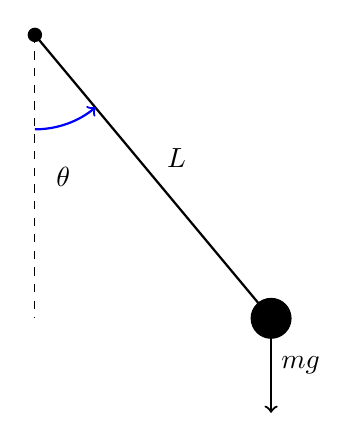
\begin{tikzpicture}[scale=1.2]
        % Draw the pivot point
        \filldraw[black] (0,0) circle (2pt);
        
        % Draw the rod
        \draw[thick] (0,0) -- (2.5,-3);
        
        % Draw the bob
        \filldraw[black] (2.5,-3) circle (6pt);
        
        % Draw the angle theta
        \draw[->,thick,blue] (0,-1) arc[start angle=-90,end angle=-50,radius=1];
        \node at (0.3,-1.5) {$\theta$};
        
        % Draw the forces
        \draw[->,thick] (2.5,-3) -- ++(0,-1) node[midway, right] {$mg$};
        
        % Draw the length of the pendulum
        \draw[dashed] (0,0) -- (0,-3);
        \node at (1.5,-1.3) {$L$};
    \end{tikzpicture}
    \caption{Pendulum Free Body Diagram}
\end{figure}
The pendulum consists of a mass $m$ attached to a rigid, massless rod of length $L$. The pendulum swings about a pivot point under the influence of gravity, which exerts a downward force $mg$ on the mass. An external torque $\tau$ acts at the pivot point itself. The angle $\theta$ represents the angular displacement of the pendulum from the vertical equilibrium position. The equation of motion for the pendulum can be derived just as before with the sum of torques acting on a body equaling the moment of inertia times its angular acceleration. The moment of inertia $J$ for a point mass at a distance $L$ from the pivot is given by $J = mL^2$. The torque generated by the gravitational force is $\tau_g = -mgL \sin{\theta}$, where the negative sign indicates that gravity acts to restore the pendulum to its equilibrium position. Thus, the equation of motion is given as
\begin{equation}
    J\ddot{\theta} = \vec{M_C} = -mgL \sin{\theta} + \tau
\end{equation}
Rearranging and substituting the moment of inertia yields
\begin{equation}
    \ddot{\theta} = \frac{\tau}{mL} - \frac{g}{L} \sin{\theta}
\end{equation}
This equation is close to the second order equations where the damping ratio is zero but it is nonlinear due to the $\sin{\theta}$ and $\cos{\theta}$ terms. In this case the system can be linearized about the equilibrium point $\theta=0$ but can also be linearized about the equilibrium point $\theta=\pi$ if the pendulum is inverted. In order to linearize the equations of motion you need to use equation \ref{e:linearize} from the linearization section. Note that in this case the matrices $A$ and $B$ are expanded out instead of using matrix notation.
\begin{equation}
    \Delta \ddot{\theta} = \frac{\partial f}{\partial \dot{\theta}} \Delta \dot{\theta} + \frac{\partial f}{\partial \theta}\Delta \theta + \frac{\partial g}{\partial \tau} \Delta \tau 
\end{equation}
where $f = -(g/L) \sin{\theta}$ and $g = \tau/(mL)$. Calculating the partial derivative and plugging into the equation above yields
\begin{equation}
    \Delta \ddot{\theta} = 0 -\frac{g}{L}cos(\theta_e)\Delta \theta + \frac{1}{mL} \Delta \tau
\end{equation}
Rearranging and dropping the $\Delta$ terms yields
\begin{equation}
    \ddot{\theta} + \frac{g}{L}cos(\theta_e)\theta = \frac{1}{mL} \tau
\end{equation}
This will now yield two separate and quite different equations depending on the equilibrium point chosen. First, if the equilibrium point is $\theta_e=0$ the equation becomes
\begin{equation}
    \ddot{\theta} + \frac{g}{L}\theta = \frac{1}{mL} \tau
\end{equation}
which is in the standard form of second order systems where ${\omega_n}^2 = g/L$ and $\zeta = 0$. The control term is $\tau = fmg$ which results in the same equation as \ref{e:second_order}. If $\theta_e=\pi$ the equation becomes
\begin{equation}
    \ddot{\theta} - \frac{g}{L}\theta = \frac{1}{mL} \tau
\end{equation}
which is again in the standard form of second order systems except that the constant term is negative which means the system is actually unstable. More on this system will be discussed in the stability section. Furthermore, the solution is also quite different and will be explored in the sections that follow.

\subsection{Characteristic and Particular Solutions to Differential Equations}

The differential equations presented in the previous section can be solved using a variety of methods. The most common methods are the characteristic and particular solution method and the Laplace transform method. The sections below will discuss both methods starting with the characteristic and particular solution method.

\subsubsection{General First Order System}

First the first order system defined above will be solved first. For a first order linear differential equation of the form presented in equation \ref{e:first_order}, the general solution is the sum of the homogeneous (characteristic) solution and a particular solution. The particular solution corresponds to the steady-state response when the forcing function $f$ is constant. In this case assume $f$ is a step function which is just a constant $f_0$. The particular solution $q_p(t)=C$ where $C$ is a constant and thus $\dot{q_p}=\dot{C}=0.$ Plugging this into equation \ref{e:first_order} gives
\begin{equation}
    0 + \sigma q_p = \sigma f_0 
\end{equation}
Thus, the particular solution for a constant input is simply $q_p = f_0$. If the forcing function is not constant then the particular solution will be a function of time and solving for the particular solution will be more difficult. Examples of this include sinusoidal forcing functions or exponentially decaying forcing functions. The solutions to these types of forcing functions can be found in many differential equations textbooks and will not be discussed here for the time being. The homogeneous solution is found by setting the forcing function to zero and solving the resulting equation assuming that $q_h(t)=Ae^{st}$. Thus, the homogeneous equation is
\begin{equation}
    \dot{q_h} + \sigma q_h = Ase^{st} + \sigma Ae^{st} = Ae^{st}(s+\sigma) = 0
\end{equation}
In the equation above the result yields 3 equations that could be equal to zero. The first is $A=0$ which is a trivial solution and thus not considered. The second is $e^{st}=0$ which is never true for any real or complex value of s. The third is $s+\sigma=0$ which is the charactertic equation for the first order system. The solution to this equation yields the characteristic root $s=-\sigma$. Thus, the homogeneous solution is
\begin{equation}
    q_h(t) = Ae^{-\sigma t}
\end{equation}
where A is a constant determined by the initial conditions. The general solution is the sum of the homogeneous and particular solutions
\begin{equation}
    q(t) = q_h(t) + q_p(t) = Ae^{-\sigma t} + f_0
\end{equation}
The constant A can be determined by the initial condition $q(0)=q_0$ which yields
\begin{equation}
    q(0) = A + f_0 = q_0 \implies A = q_0 - f_0
\end{equation}
Thus, the final solution to the first order system is 
\begin{equation}
    q(t) = q_0 - f_0 + Ae^{-\sigma t}
\end{equation}
or more simply
\begin{equation}
    q(t) = f_0 + (q_0 - f_0)e^{-\sigma t}
\end{equation}
In the case of the car example the solution would be
\begin{equation}
    v(t) = \frac{F_0}{c} + \left(v_0 - \frac{F_0}{c}\right)e^{-\frac{c}{m}t}
\end{equation}
noting that $\sigma = c/m$,$F_0 = cf_0$ and $v_0$ is the initial velocity of the car. Typically for these types of systems the initial velocity is zero so the equation simplifies to
\begin{equation}\label{e:first_order_solution}
    v(t) = \frac{F_0}{c}\left(1 - e^{-\frac{c}{m}t}\right)
\end{equation}
which shows that the car will asymptotically approach a steady state velocity of $F_0/c$. This will be plotted later in the time response section for open loop analysis.

\subsubsection{General Second Order Systems}

The solution to second order systems is quite complex given the nature of solving a second order differential equation. The general solution is again the sum of the homogeneous and particular solutions and assume the initial conditions are zero. The major difficulty with second order systems is that the solution to the homogenous characteristic eqaution can be real, repeated or imaginary roots. The roots effect the overall solution and will be discussed later. To start the particular solution is very simple and is again found by assuming a constant forcing function $f_0$ such that $q_p(t)=C$ where $C$ is a constant and thus $\dot{q_p}=\dot{C}=0$ and $\ddot{q_p}=\ddot{C}=0$. Plugging this into equation \ref{e:second_order} gives the eqaution below:

\begin{equation}
    0 + 0 + {\omega_n}^2 q_p = {\omega_n}^2 f_0
\end{equation}
Thus, the particular solution for a constant input is simply $q_p = f_0$. If the forcing function is not constant then the particular solution will be a function of time and solving for the particular solution will be more difficult. Examples of this include sinusoidal forcing functions or exponentially decaying forcing functions. The solutions to these types of forcing functions can be found in many differential equations textbooks and will not be discussed here for the time being. The homogeneous solution is found by setting the forcing function to zero and solving the resulting equation assuming that $q_h(t)=Ae^{st}$. Thus the homogeneous equation is
\begin{equation}
    \begin{matrix}
    \ddot{q_h} + 2\zeta \omega_n \dot{q_h} + {\omega_n}^2 q_h = 0 \\
    A s^2 e^{st} + 2\zeta \omega_n A s e^{st} + {\omega_n}^2 A e^{st} = 0 \\
    Ae^{st}(s^2 + 2\zeta \omega_n s + {\omega_n}^2) = 0
    \end{matrix}
\end{equation}
In the equation above the result yields 3 equations that could be equal to zero. The first is $A=0$ which is a trivial solution and thus not considered. The second is $e^{st}=0$ which is never true for any real or complex value of s. The third is $s^2 + 2\zeta \omega_n s + {\omega_n}^2 = 0$ which is the charactertic equation for the second order system. The solution to this equation yields the characteristic roots which as stated above can have real, repeated or imaginary roots. The characteristic roots are found using the quadratic formula and are given as
\begin{equation}
    s = -\zeta \omega_n \pm \omega_n \sqrt{\zeta^2 - 1}
\end{equation}
Note that if ${\omega_n}^2$ is negative, as is the case with the unstable $C_{m\alpha}$ of the F-16 or the inverted pendulum, the characteristic equation becomes $s^2 + 2\zeta \omega_n s - \omega_n^2 = 0$ which results in roots of
\begin{equation}
    s = -\zeta \omega_n \pm \omega_n \sqrt{\zeta^2 + 1}
\end{equation}
which is almost the same but notice the plus sign in front of the $\zeta^2$ term. In this case the roots are always real and distinct. It is possible to have complex roots if the damping ratio $\zeta$ is negative but this is not a common case and will not be discussed here. The nature of the roots depends on the value of the damping ratio $\zeta$ as well as the sign of $\omega_n^2$. The three cases for ${\omega_n}^2>0$ are underdamped ($0 \leq \zeta<1$), critically damped ($\zeta=1$), and overdamped ($\zeta>1$). Each case will be discussed below. Note that for the case where ${\omega_n}^2<0$ the roots are always real and distinct which has a similar solution to the overdamped case.
\begin{itemize}
    \item {\bf Underdamped ($0 \leq \zeta<1$)}: In this case, the roots are complex conjugates ($s_{12}=-\zeta w_n \pm \omega_d j$) where $\omega_d = \omega_n\sqrt{1 - \zeta^2}$, leading to oscillatory behavior. Note that this case also applies to the edge case where the damping ratio $\zeta$ is zero. The homogeneous solution is given by:
    \begin{equation}
        q_h(t) = e^{-\zeta \omega_n t} \left( A_1 \cos(\omega_d t) + A_2 \sin(\omega_d t) \right)
    \end{equation}
    where $\omega_d = \omega_n \sqrt{1 - \zeta^2}$ is the damped natural frequency, and $A_1$ and $A_2$ are constants determined by initial conditions.

    \item {\bf Critically Damped ($\zeta=1$)}: In this case, the roots are real and repeated ($s_{12}=-\omega_n$). The homogeneous solution is given by:
    \begin{equation}
        q_h(t) = (A_1 + A_2 t) e^{-\omega_n t}
    \end{equation}

    \item {\bf Overdamped ($\zeta>1$ or ${\omega_n}^2<0)$}: In this case, the roots are real and distinct ($s_{12}=-\zeta \omega_n \pm \omega_n \sqrt{\zeta^2-1}$) or ($s_{12}=-\zeta \omega_n \pm \omega_n \sqrt{\zeta^2+1}$). The homogeneous solution is given by:
    \begin{equation}
        q_h(t) = A_1 e^{s_1 t} + A_2 e^{s_2 t}
    \end{equation}
\end{itemize}
The general solution is the sum of the homogeneous and particular solutions
\begin{equation}
    q(t) = q_h(t) + q_p(t) = q_h(t) + f_0
\end{equation}
The constants $A_1$ and $A_2$ can be determined by the initial conditions $q(0)=q_0$ and $\dot{q}(0)=\dot{q_0}$. The final solution will depend on the damping ratio $\zeta$ and the initial conditions. For the case where the initial conditions are zero the final solutions for each case are shown below.
\begin{itemize}
    \item {\bf Underdamped ($0 \leq \zeta<1$)} Note the solution is still valid if $\zeta=0$:
    \begin{equation}
        q(t) = f_0 \left( 1 - e^{-\zeta \omega_n t} \left( \cos(\omega_d t) + \frac{\zeta}{\sqrt{1-\zeta^2}} \sin(\omega_d t) \right) \right)
    \end{equation}
    \item {\bf Critically Damped ($\zeta=1$)}:
    \begin{equation}
        q(t) = f_0 \left( 1 - (1 + \omega_n t) e^{-\omega_n t} \right)
    \end{equation}
    \item {\bf Overdamped ($\zeta>1$ or ${\omega_n}^2<0$)}:
    \begin{equation}
        q(t) = f_0 \left( 1 - \frac{s_2 e^{s_1 t} - s_1 e^{s_2 t}}{s_2 - s_1} \right)
    \end{equation}
\end{itemize}
In the case of the mass-spring-damper example, recall that $f_0=F_0/k$, $\omega_n = \sqrt{k/m}$, and $\zeta = c/(2\sqrt{mk})$.

\subsubsection{Special Case of Natural Frequency Equal to Zero}

As was shown in the special case of the car where no restoring force existed, the natural frequency was equal to zero. In this case the general equation of motion was $\ddot{q} + \sigma \dot{q} = \sigma f$. The solution to this equation is different given the characteristic equation is $s^2+\sigma s=0$ which has two roots of $s=0$ and $s=-\sigma$. The homogeneous solution in this case is given as 
\begin{equation}
    q_h(t) = A_1 + A_2 e^{-\sigma t}
\end{equation}
For the particular solution again assume a constant forcing function $f_0$ such that $q_p(t)=C t$ where $C$ is a constant and thus $\dot{q_p}=C$ and $\ddot{q_p}=0$. Plugging this into the equation of motion gives
\begin{equation}
    0 + \sigma C = \sigma f_0
\end{equation}
and then $C = f_0$. Thus, the particular solution is $q_p(t)=f_0 t$ and the general solution is
\begin{equation}
    q(t) = A_1 + A_2 e^{-\sigma t} + f_0 t
\end{equation} 
The constants $A_1$ and $A_2$ can be determined by the initial conditions $q(0)=q_0$ and $\dot{q}(0)=\dot{q_0}$. For the case where the initial conditions are zero the final solution is given as 
\begin{equation}
    q(t) = f_0 t - \frac{f_0}{\sigma} (1 - e^{-\sigma t})
\end{equation}
In the case of the car example, recall that $f_0 = F_0/c$ and $\sigma = c/m$. Plugging those values into the equation yields 
\begin{equation}
    x(t) = \frac{F_0}{c} t - \frac{F_0 m}{c^2} (1 - e^{-c/m t})
\end{equation}
This result is intuitive because it states that if a constant force to the car is applied, the car will initially accelerate but then reach a constant velocity due to the drag force. This is different than the case of the quadcopter/satellite example where the angle will continue to accelerate. Note that $\dot{x} = v$. Applying a derivative to the equation above yields the same result as equation the equation for velocity
\begin{equation}\label{e:position_car_solution}
    \dot{x}(t) = v(t) = \frac{F_0}{c} - 0 - \frac{c}{m}\frac{F_0 m}{c^2} e^{-c/m t} = \frac{F_0}{c}\left(1 - e^{-\frac{c}{m}t}\right)
\end{equation}
This is a good check for the budding controls engineer to ensure that the math is correct. 

\subsubsection{Special Case of Natural Frequency and Damping Ratio Equal to Zero}

As was shown in the special case of the satellite/quadcopter where no restoring moment or damping moment existed, the natural frequency and damping ratio were both equal to zero. In this case the general equation of motion was $\ddot{q} = f$. The solution to this equation is different given the characteristic equation is simply $s^2=0$ which has a repeated root of $s=0$. The homogeneous solution is then given as
\begin{equation}
    q_h(t) = A_1 + A_2 t
\end{equation}
since $e^{0t}=1$. The particular solution is again $q_p(t)=(A_0/2)t^2$ where $A_0$ is a constant. Plugging this into the equation of motion gives
\begin{equation}
    \ddot{q_p} = A_0 = f_0
\end{equation}
Thus, the particular solution is $q_p(t)=f_0 t^2/2$ and the general solution is
\begin{equation}
    q(t) = A_1 + A_2 t + \frac{f_0}{2} t^2
\end{equation}
The constants $A_1$ and $A_2$ can be determined by the initial conditions $q(0)=q_0$ and $\dot{q}(0)=\dot{q_0}$. For the case where the initial conditions are zero the final solution is given as 
\begin{equation}
    q(t) = \frac{f_0}{2} t^2
\end{equation}
In the case of the satellite/quadcopter example, recall that $f_0 = \frac{2F_0 d}{J}$. This result is intuitive because it states that if a constant force to the thrusters/propellors is applied, the angle of the satellite/quadcopter will increase quadratically over time. That is, the system will continue to accelerate until it runs out of fuel or the thrusters are turned off. In the case of the quadcopter, if the propellors return to symmetric thrust the quadcopter will stop accelerating and maintain a constant angular velocity. In practice of course the quadcopter will have some damping due to air resistance and the satellite will have some damping due to magnetic torques and other effects. However, these effects are typically small and can be ignored for control purposes.

\subsection{Laplace Solutions}

Another method to solve linear differential equations is the Laplace transform method. The Laplace transform converts a time-domain differential equation into an algebraic equation in the s-domain, which can be easier to manipulate and solve. The Laplace domain and algebraic equations are very useful for control system dynamics and every undergraduate controls engineer should learn its fundamentals. The Laplace transform of a function $f(t)$ is defined as 
\begin{equation}
    F(s) = \mathcal{L}\{f(t)\} = \int_0^{\infty} f(t) e^{-st} dt
\end{equation}
where $s$ is a complex variable similar to the $s$ in the $Ae^{st}$ equations discussed earlier. The inverse Laplace transform is given by 
\begin{equation}
    f(t) = \mathcal{L}^{-1}\{F(s)\} = \frac{1}{2\pi j} \lim_{T \to \infty} \int_{\gamma - jT}^{\gamma + jT} F(s) e^{st} ds
\end{equation}
where $\gamma$ is a real number such that all singularities of $F(s)$ are to the left of the line $Re(s) = \gamma$. Note that these integrals are very complex and not typically solved by hand but rather looked up in a table of Laplace transforms. Some common Laplace transforms are shown below
\renewcommand{\arraystretch}{1.5} % Increase row spacing by 1.5x
\begin{table}[H]
\centering
\begin{tabular}{|c|c|c|}
\hline
Time Domain $f(t)$ & Laplace Transform $\mathcal{L}\{f(t)\}$ & Description \\
\hline
$u(t)$ & $\frac{1}{s}$ & Unit step \\
$t$ & $\frac{1}{s^2}$ & Ramp \\
$e^{at}$ & $\frac{1}{s-a}$ & Exponential \\
$sin(at)$ & $\frac{a}{s^2 + a^2}$ & Sine \\
$cos(at)$ & $\frac{s}{s^2 + a^2}$ & Cosine \\
$t^2$ & $\frac{2}{s^3}$ & Quadratic \\
$te^{at}$ & $\frac{1}{(s-a)^2}$ & Repeated Root \\
$e^{at}sin(bt)$ & $\frac{b}{(s-a)^2 + b^2}$ & Underdamped Sine \\
$e^{at}cos(bt)$ & $\frac{s-a}{(s-a)^2 + b^2}$ & Underdamped Cosine \\
$\int f(t) dt$ & $\frac{F(s)}{s}$ & Integral \\
$\dot{f}(t)$ & $sF(s) - f(0)$ & First derivative \\
$\ddot{f}(t)$ & $s^2F(s) - sf(0) - \dot{f}(0)$ & Second derivative \\
\hline
\end{tabular}
\caption{Common Laplace transforms}
\end{table}
\renewcommand{\arraystretch}{1} % Reset 
where $u(t)$ is the unit step function where $u(t)=0$ for $t<0$ and $u(t)=1$ for $t\geq0$. The undergraduate student may look at these equations and wonder how exactly these functions are helpful. To illustrate their usefulness the first and second order systems defined above will be solved using the Laplace transform method.

\subsubsection{General First Order Systems}

Taking the Laplace transform of equation \ref{e:first_order} and assuming zero initial conditions gives 
\begin{equation}
    sQ(s) + \sigma Q(s) = \sigma F(s)
\end{equation}
where $Q(s)$ is the Laplace transform of $q(t)$ and $F(s)$ is the Laplace transform of $f(t)$. Rearranging gives the equation below
\begin{equation}
    \frac{Q(s)}{F(s)} = G(s) = \frac{\sigma}{(s+\sigma)}
\end{equation}
The function $G(s)$ is called the transfer function of the system and is a very important function in control systems. The transfer function relates the output of the system $Q(s)$ to the input of the system $F(s)$ in the Laplace domain. The transfer function can be used to analyze the stability and performance of the system. The transfer function can also be used to design controllers for the system which will be discussed later. Let's now assume that the forcing function is a step function such that $f(t)=f_0u(t)$ where $u(t)$ is the unit step function. The Laplace transform of a step function is $F(s)=f_0/s$. Plugging this into the equation above gives
\begin{equation}
    Q(s) = G(s)F(s) = \frac{\sigma}{s+\sigma}\frac{f_0}{s} = \frac{\sigma f_0}{s(s+\sigma)}
\end{equation}
The solution to the equation above can be found by taking the inverse Laplace transform. However, the equation above is not in the standard table of Laplace transforms. Thus partial fraction decomposition is needed to get $Q(s)$ into a form that can be used for inverse Laplace. The equation can be rewritten using partial fractions as
\begin{equation}
    Q(s) = \frac{\sigma f_0}{s(s+\sigma)} = \frac{A}{s} + \frac{B}{s+\sigma}
\end{equation}
where $A$ and $B$ are constants to be determined. Multiplying both sides by the denominator on the left side gives
\begin{equation}
    \sigma f_0 = A(s+\sigma) + Bs
\end{equation}
Setting $s=0$ gives $A=\sigma f_0/\sigma = f_0$. Setting $s=-\sigma$ gives $B=-\sigma f_0/\sigma = -f_0$. Thus, the equation can be rewritten as
\begin{equation}
    Q(s) = \frac{f_0}{s} - \frac{f_0}{s+\sigma}
\end{equation}
Taking the inverse Laplace transform gives
\begin{equation}
    q(t) = f_0 - f_0 e^{-\sigma t} = f_0(1 - e^{-\sigma t})
\end{equation}
substituting back in the values for $\sigma$ and $f_0$ gives
\begin{equation}
    v(t) = \frac{F_0}{c}(1 - e^{-\frac{c}{m}t})
\end{equation}
which is the same solution as derived using the characteristic and particular solution method assuming zero initial conditions as given by equation \ref{e:first_order_solution}.

\subsubsection{General Second Order Systems}

Taking the Laplace transform of equation \ref{e:second_order} and assuming zero initial conditions gives
\begin{equation}
    s^2 Q(s) + 2\zeta \omega_n s Q(s) + {\omega_n}^2 Q(s) = {\omega_n}^2 F(s)
\end{equation}
Rearranging just as before gives the equation below 
\begin{equation}
    \frac{Q(s)}{F(s)} = G(s) = \frac{{\omega_n}^2}{s^2 + 2\zeta \omega_n s + {\omega_n}^2}
\end{equation}
where again $G(s)$ is the transfer function of the system. Let's again assume that the forcing function is a step function such that $f(t)=f_0u(t)$. Plugging the Laplace transform of $F(s)$ just as before gives
\begin{equation}
    Q(s) = G(s)F(s) = \frac{{\omega_n}^2}{s^2 + 2\zeta \omega_n s + {\omega_n}^2}\frac{f_0}{s} = \frac{{\omega_n}^2 f_0}{s(s^2 + 2\zeta \omega_n s + {\omega_n}^2)}
\end{equation}
The solution to the equation above again can be found by taking the inverse Laplace transform. However, again the equation above is not in the standard table of Laplace transforms. Thus partial fraction decomposition is needed to get $Q(s)$ into a form that can be used for inverse Laplace. The equation can be rewritten using partial fractions as
\begin{equation}
    Q(s) = \frac{{\omega_n}^2 f_0}{s(s^2 + 2\zeta \omega_n s + {\omega_n}^2)} = \frac{A}{s} + \frac{Bs + C}{s^2 + 2\zeta \omega_n s + {\omega_n}^2}
\end{equation}
where $A$, $B$ and $C$ are constants to be determined. Multiplying both sides by the denominator on the left side gives
\begin{equation}
    {\omega_n}^2 f_0 = A(s^2 + 2\zeta \omega_n s + {\omega_n}^2) + (Bs + C)s
\end{equation}
Setting $s=0$ gives $A={\omega_n}^2 f_0/{\omega_n}^2 = f_0$. Setting $s=j\omega_n(-\zeta + \sqrt{\zeta^2 - 1})$ and $s=j\omega_n(-\zeta - \sqrt{\zeta^2 - 1})$ gives two equations that can be solved simultaneously to find $B$ and $C$. The final results are $B=-f_0$ and $C=-2\zeta \omega_n f_0$. Thus, the equation can be rewritten as
\begin{equation}
    Q(s) = \frac{f_0}{s} - \frac{f_0 s + 2\zeta \omega_n f_0}{s^2 + 2\zeta \omega_n s + {\omega_n}^2}
\end{equation}
The first term of the equation is simply the Laplace transform of a step function. The second term can be solved using the table of Laplace transforms. The final solution depends on the value of the damping ratio $\zeta$ just as before. The final solutions for each case assuming zero initial conditions are shown below. It is left to the reader to verify that these solutions match those derived using the characteristic and particular solution method. For the case when $\zeta=0$ the inverse laplace is simply a sine or cosine while the the general underdamped solution is solved by completing the square in the denominator and using the Laplace transform of the underdamped sine and cosine functions. The critically damped and overdamped solutions are solved using the Laplace transforms of repeated roots and real distinct roots respectively.
\begin{itemize}
    \item {\bf Underdamped ($0 \leq \zeta<1$)}:
    \begin{equation}
        q(t) = f_0 \left( 1 - e^{-\zeta \omega_n t} \left( \cos(\omega_d t) + \frac{\zeta}{\sqrt{1-\zeta^2}} \sin(\omega_d t) \right) \right)
    \end{equation}
    \item {\bf Critically Damped ($\zeta=1$)}:
    \begin{equation}
        q(t) = f_0 \left( 1 - (1 + \omega_n t) e^{-\omega_n t} \right)
    \end{equation}
    \item {\bf Overdamped ($\zeta>1$ or ${\omega_n}^2<0)$}:
    \begin{equation}
        q(t) = f_0 \left( 1 - \frac{s_2 e^{s_1 t} - s_1 e^{s_2 t}}{s_2 - s_1} \right)
    \end{equation}
\end{itemize}
Notice again that the solutions are the same as those derived using the characteristic and particular solution method assuming zero initial conditions. It is possible that the undergraduate engineer still does not see the usefulness of the Laplace transform method. The true power of the Laplace transform method is in the transfer function. The transfer function can be used to analyze the stability and performance of the system as well as design controllers for the system which will be discussed in the sections below.

\subsubsection{Special Case of Natural Frequency Equal to Zero}

As was shown in the special case of the car where no restoring force existed, the natural frequency was equal to zero. In this case the general equation of motion was $\ddot{q} + \sigma \dot{q} = \sigma f$. Taking the laplace transform of this equation and assuming zero initial conditions gives
\begin{equation}
    s^2 Q(s) + \sigma s Q(s) = \sigma F(s)
\end{equation}
Rearranging gives the equation below
\begin{equation}
    \frac{Q(s)}{F(s)} = G(s) = \frac{\sigma}{s(s+\sigma)}
\end{equation}
where again $G(s)$ is the transfer function of the system. Notice that this is identical to the first order transfer function multiplied by an additional $1/s$ term. This is because the second order system with zero natural frequency is simply the integral of the first order system. That is $x(t) = \int v(t) dt$. In the Laplace domain this means that $X(s) = \frac{1}{s}V(s)$ or if we let $\dot{x} = v(t)$ the lapace transform would result in $sX(s) = V(s)$. This is where the Laplace transform method really shines. The transfer function can be manipulated easily in the Laplace domain to find relationships between different variables. Differential equations in the time domain can be difficult to manipulate but in the Laplace domain they are simply algebraic equations. Let's again assume that the forcing function is a step function such that $f(t)=f_0u(t)$. Plugging the Laplace transform of $F(s)$ just as before gives
\begin{equation}
    Q(s) = G(s)F(s) = \frac{\sigma}{s(s+\sigma)}\frac{f_0}{s} = \frac{\sigma f_0}{s^2(s+\sigma)}
\end{equation}
The solution to the equation above can be found by taking the inverse Laplace transform. However, again the equation above is not in the standard table of Laplace transforms. Thus partial fraction decomposition is needed to get $Q(s)$ into a form that can be used for inverse Laplace. The equation can be rewritten using partial fractions as
\begin{equation}
    Q(s) = \frac{\sigma f_0}{s^2(s+\sigma)} = \frac{A}{s} + \frac{B}{s^2} + \frac{C}{s+\sigma}
\end{equation}
where $A$, $B$ and $C$ are constants to be determined. Multiplying both sides by the denominator on the left side gives
\begin{equation}
    \sigma f_0 = A s (s+\sigma) + B (s+\sigma) + C s^2
\end{equation}
Setting $s=0$ gives $\sigma f_0 = \sigma B$ and $B = f_0$. Setting $s=-\sigma$ gives $C \sigma^2=\sigma f_0$ and thus $C=f_0/\sigma$. Setting $s=1$ gives 
\begin{equation}
    \begin{matrix}
        \sigma f_0 = A(\sigma+1)+f_0(\sigma+1)+f_0/\sigma \\
        \sigma^2 f_0 = A\sigma(\sigma+1)+f_0\sigma(\sigma+1)+f_0 \\
        (\sigma^2 - 1) f_0 = (\sigma+1)(\sigma-1)f_0 = A\sigma(\sigma+1) +f_0\sigma(\sigma+1)\\
        \sigma f_0 - f_0 = A \sigma + f_0 \sigma \\
        A = -f_0/\sigma
    \end{matrix}
\end{equation}
Plugging in these values for A, B, and C gives        
\begin{equation}
    Q(s) = -\frac{f_0}{\sigma s} + \frac{f_0}{s^2} + \frac{f_0}{\sigma}\frac{1}{s+\sigma}
\end{equation}
Taking the inverse Laplace transform gives
\begin{equation}
    q(t) = -\frac{f_0}{\sigma} + f_0 t + \frac{f_0}{\sigma} e^{-\sigma t} = f_0 t - \frac{f_0}{\sigma}(1 - e^{-\sigma t})
\end{equation}
which is the same result shown previously. Taking the derivative of the equation above gives the same result as the velocity equation shown previously. The budding controls engineer may think that the method of partial fractions and inverse Laplace transform is tedious and not worth the effort. However, the true power of the Laplace transform method is in the transfer function. The transfer function can be used to analyze the stability and performance of the system as well as design controllers for the system which will be discussed in detail in Chapter \ref{s:control_systems}.

\subsubsection{Special Case of Natural Frequency and Damping Ratio Equal to Zero}

As was shown in the special case of the satellite/quadcopter where no restoring moment or damping moment existed, the natural frequency and damping ratio were both equal to zero. In this case the general equation of motion was $\ddot{q} = f$. Taking the Laplace transform of this equation and assuming zero initial conditions gives
\begin{equation}
    s^2 Q(s) = F(s)
\end{equation}
Rearranging gives the equation below
\begin{equation}
    \frac{Q(s)}{F(s)} = G(s) = \frac{1}{s^2}
\end{equation}
where again $G(s)$ is the transfer function of the system. Let's again assume that the forcing function is a step function such that $f(t)=f_0u(t)$. Plugging the Laplace transform of $F(s)$ just as before gives
\begin{equation}
    Q(s) = G(s)F(s) = \frac{1}{s^2}\frac{f_0}{s} = \frac{f_0}{s^3}
\end{equation}
The solution to the equation above can be found by taking the inverse Laplace transform. The equation above is in the standard table of Laplace transforms and the inverse Laplace transform is given as 
\begin{equation}
    q(t) = \frac{f_0}{2}t^2
\end{equation}
which is the same solution as derived using the characteristic and particular solution method assuming zero initial conditions. In the case of the satellite example, recall that $f_0 = \frac{2F_0 d}{J}$.

\subsection{Open Loop Time Response}

Now that the solutions to the first and second order systems have been derived using both the characteristic and particular solution method as well as the Laplace transform method, the time response of these systems can be analyzed. The time response of a system is the output of the system as a function of time given a specific input. The time response can be used to analyze the stability and performance of the system. 

\subsubsection{Position and Velocity Response of a Car}

First, let's plot the time response of the first order system given by equation \ref{e:first_order_solution} as well as the second order solution given by equation \ref{e:position_car_solution}. The parameters for the system are chosen to be $F_0=1000~N$, $c=50~Ns/m$, and $m=1000~kg$. The initial velocity and position are assumed to be zero. In order to show the time response however, 3 different curves will be placed on the graph. The first will be the analytic solution to the first and second order system, the second is the Laplace transform solution using the control systems toolbox in Python and the last is the numerical integration of the equations of motion. The python code used to generate this is shown in the Figure below and also available on \href{https://github.com/cmontalvo251/Python/blob/master/controls/first_order_system.py}{GitHub}.
\begin{figure}[H]
\centering
\begin{minipage}{0.48\textwidth}
\centering
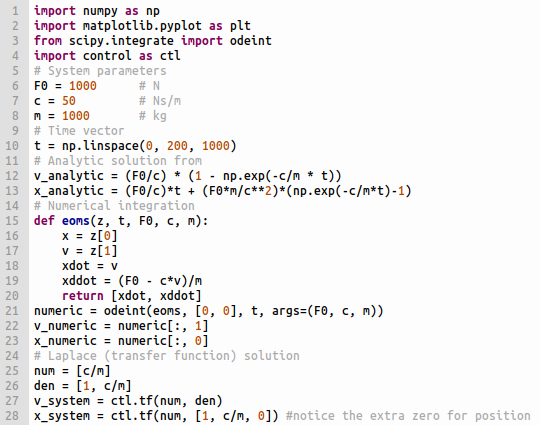
\includegraphics[width=\linewidth]{Figures/car_code_1.png}
\end{minipage}\hfill
\begin{minipage}{0.48\textwidth}
\centering
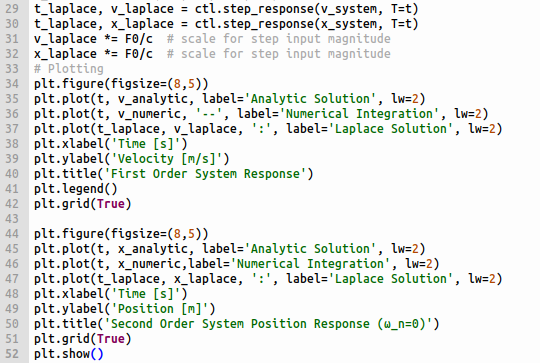
\includegraphics[width=\linewidth]{Figures/car_code_2.png}
\end{minipage}
\caption{Python code to generate the time response of a car}
\label{f:car_code}
\end{figure}
Note the code is commented to help the reader understand what is happening. Note the benefit of using the control systems toolbox in Python. The time response can be generated by first creating the transfer function and then applying a step to the transfer function. This will come in handy later when it is necessary to apply a control system to the transfer function before inversing back to the time domain. The numerical integration is also useful when the equations of motion are known and the control system designer wants to work in the time doman rather than the laplace domain. It's also very helpful when the system is non-linear since transfer functions only work for linear systems. All three methods have their pros and cons. The numerical integration is done using the scipy.integrate.odeint function which is a simple way to numerically integrate ordinary differential equations. The results of the time response are shown in Figure \ref{f:car_response}.
\begin{figure}[H]
\centering
\begin{minipage}{0.48\textwidth}
\centering
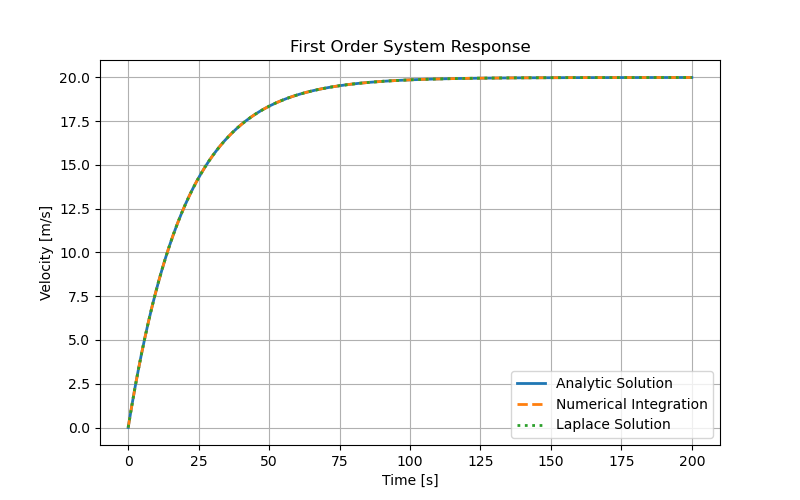
\includegraphics[width=\linewidth]{Figures/car_velocity_response.png}
\end{minipage}\hfill
\begin{minipage}{0.48\textwidth}
\centering
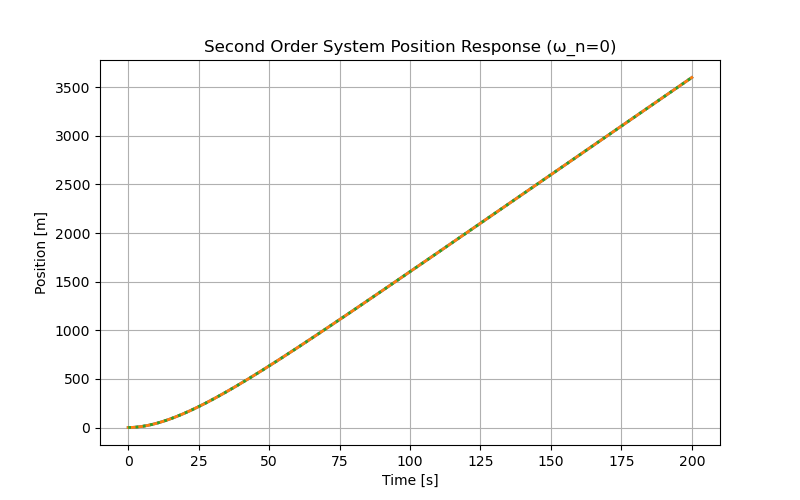
\includegraphics[width=\linewidth]{Figures/car_position_response.png}
\end{minipage}
\caption{Time response of the position (right) and velocity (left) of a car}
\label{f:car_response}
\end{figure}
\noindent The time response shows that the velocity of the car asymptotically approaches a steady state value of $F_0/c = 20~m/s$. The time constant of the system is $\tau = m/c = 20~s$. The time constant is the time it takes for the system to reach 63.2\% of its steady state value. The settling time $T_s=4\tau$ is the time the system takes to get within 2\% of its final value. In this case that is $80~s$. The time response can be used to analyze the stability and performance of the system. In this case, the system is stable and the performance is acceptable given the parameters chosen. However, examining the position of the car shows that the position will continue to increase linearly over time. This is because the car is moving at a constant velocity. The position of the car will not reach a steady state value but rather continue to increase linearly over time. This is an example of a marginally stable system. The velocity of the car is stable while the position of the car is marginally stable.

\subsubsection{Position of a Mass Spring Damper}

Simulating the mass spring damper is very similar to the car example. The parameters for the system are chosen to be $F_0=1000~N$, $k=2000~N/m$, $c=50~Ns/m$, and $m=100~kg$. The initial position and velocity are assumed to be zero. The python code used to generate this is shown in the Figure below and also available on \href{https://github.com/cmontalvo251/Python/blob/master/controls/mass_spring_damper.py}{GitHub}. 
\begin{figure}[H]
\centering
\begin{minipage}{0.48\textwidth}
\centering
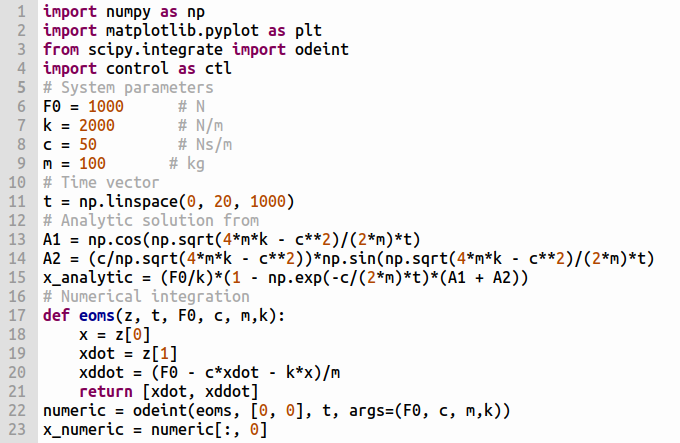
\includegraphics[width=\linewidth]{Figures/mass_spring_damper_code_1.png}
\end{minipage}\hfill
\begin{minipage}{0.48\textwidth}
\centering
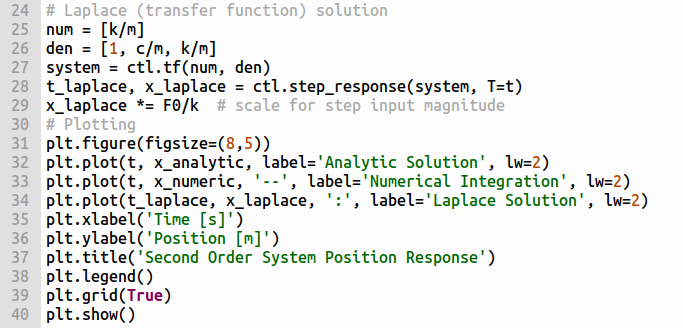
\includegraphics[width=\linewidth]{Figures/mass_spring_damper_code_2.png}
\end{minipage}
\caption{Python code to generate the time response of a mass spring damper}
\label{f:mass_spring_damper_code}
\end{figure}
Note the code is commented to help the reader understand what is happening. Again, the simulation is run by integrating the equations of motion, applying a step response to the transfer function and also plotting the analytic solution. The results of the time response are shown in Figure \ref{f:mass_spring_damper_response}.
\begin{figure}[H]
\centering
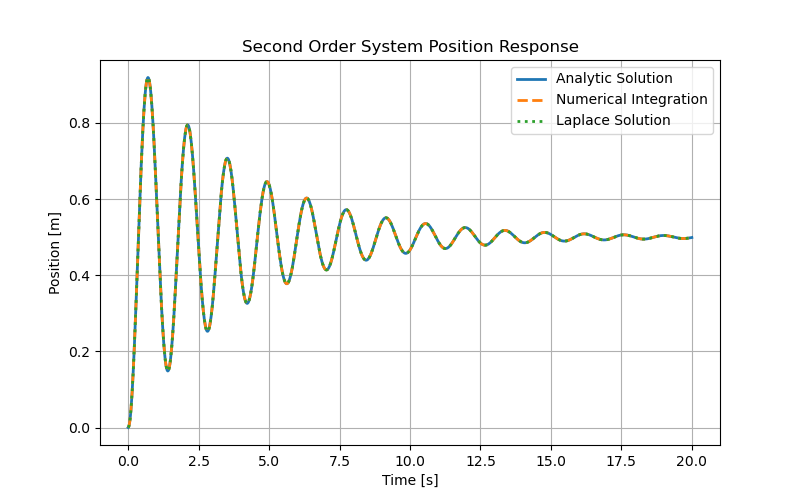
\includegraphics[width=0.8\linewidth]{Figures/mass_spring_damper_response.png}
\caption{Time response of the position of a mass spring damper}
\label{f:mass_spring_damper_response}
\end{figure}
\noindent The time response shows that the position of the mass spring damper reaches a steady state value of $F_0/k = 0.5~m$. The time constant of the system is $\tau = 2m/c = 4~s$. The natural frequency of the system is $\omega_n = \sqrt{k/m} = 4.47~rad/s$. The damping ratio of the system is $\zeta = c/(2 m\omega_n) = 0.056 (underdamped)$. The settling time $T_s=4/(\zeta \omega_n)$ is the time the system takes to get within 2\% of its final value. In this case that is $16~s$. Notice that $T_s=4\tau$ where again $\tau = 4~s$. The time response can be used to analyze the stability and performance of the system. In this case, the system is stable and the performance is acceptable given the parameters chosen. Here are some useful equations for natural frequency, settling time and other second order parameters.
\begin{equation}
    \begin{matrix}
    \omega_n = \sqrt{\frac{k}{m}} & T_s = \frac{4}{\zeta \omega_n} & \tau = \frac{2m}{c} \\
    \zeta = \frac{c}{2m\omega_n} & \omega_d = \omega_n \sqrt{1-\zeta^2} & T_s = 4\tau \\
    \omega_n = 2\pi f & f = \frac{1}{T} & \tau = \frac{1}{\zeta \omega_n} 
    \end{matrix}
\end{equation}

\subsubsection{Attitude of a Satellite or Quadcopter}

\subsubsection{Pitch Response of an Aircraft}

\subsubsection{Pitch Response of a Rocket}

\subsubsection{Angle of an Inverted Pendulum}

\subsection{Stability}

Stability of open or even closed loop systems is an important concept in control systems. An open loop system is stable if the output of the system remains bounded for a bounded input. In other words, if the input to the system is a step function, the output of the system will reach a steady state value and not diverge to infinity. The stability of a system can be analyzed using the characteristic equation of the system which was shown in the solution to multiple differential equations. The astute reader will have also noticed that the denominator of the transfer function is identical to the characteristic equation. The roots of the characteristic equation are often called the poles of the system and can be used interchangeably. Thus, the benefit of a transfer function is that stability can be ascertained immediately by looking at the denominator of the transfer function. In the Chapter on feedback control it will be shown that control systems in the laplace domain can be applied by simply multiplying different control systems and examining the resulting closed loop transfer function for stability. When designing controllers in the time domain it is almost impossible to gaurantee closed loop stability. However, with transfer functions, after a bit of algebraic manipulation stability can be ascertained. 

So what do the poles or roots of the characteristic equation tell you? Remember that the general soltion to a differential equation is $q(t) = Ae^{st}$. The value of $s$, the roots, the poles, tell whether the system will oscillate, decay or extend off to infinity. The location of the poles in the complex plane determines the stability of the system. If all poles have negative real parts, the system is stable. This would results in an equation like $e^{-st}$ where that term tends to 0 as $t \rightarrow \infty$. If any pole has a positive real part, the system is unstable. If any pole has a real part equal to zero, the system is marginally stable. Marginal stability is defined as a system that neither grows nor decays but rather oscillates indefinitely or increases but not faster than a linear term. This would result in an equation like $e^{j\omega t}$  or $f_0 t$ which is a sine/cosine function or linear term. The imaginary part of the pole determines the frequency of oscillation. The real part of the pole determines the rate of decay or growth. A pole with a large negative real part will result in a fast decay while a pole with a small negative real part will result in a slow decay. A pole with a large positive real part will result in a fast growth while a pole with a small positive real part will result in a slow growth. The sections that follow examine the transfer functions of the systems examined earlier and determine their stability. The equations below summarize the stability criteria.
\begin{itemize}
    \item {\bf Stable}: All poles have negative real parts. $Re(s) < 0$
    \item {\bf Unstable}: Any pole has a positive real part. $Re(s) > 0$
    \item {\bf Marginally Stable}: Any pole has a real part equal to zero. $Re(s) = 0$
\end{itemize}

\subsubsection{Position and Velocity of a Car}

As derived earlier the transfer function for the position of the car is given as 
\begin{equation}
    \frac{X(s)}{F(s)}= G(s) = \frac{\sigma}{s(s+\sigma)}
\end{equation}
recall also that the time domain solution to this system due to a step function was given as 
\begin{equation}
    x(t) = f_0 t - \frac{f_0}{\sigma} (1 - e^{-\sigma t})
\end{equation}
Plotted in the time domain the system accelerated and then attained a constant velocity. The poles of the system are located at $s=0$ and $s=-\sigma$. The pole at $s=-\sigma$ has a negative real part and thus is stable. This is due to the $1/(s+\sigma)$ term which translates to the $e^{-\sigma t}$ term in the time domain. The pole at $s=0$ has a real part equal to zero and thus is marginally stable as given by the $1/s$ term in the laplace domain and the $f_0 t$ term in the time domain. The marginal stability is apparent because the position of the car will continue to increase linearly over time due to the constant velocity. However, the velocity of the car will reach a steady state value and not diverge to infinity. Thus, the system is considered stable for velocity. Remember the transfer function for velocity is found by simply multiplying the position transfer function by $s$ or taking the derivative in the time domain. The transfer function for velocity is given as
\begin{equation}
    \frac{V(s)}{F(s)}= G(s) = \frac{\sigma}{s+\sigma}
\end{equation}
while the time domain solution to this system due to a step function was given as
\begin{equation}
    v(t) = f_0 (1 - e^{-\sigma t})
\end{equation}
The pole of the velocity system is located at $s=-\sigma$ again from the $1/(s+\sigma)$ term in the laplace domain and the $e^{-\sigma t}$ term in the time domain. The pole has a negative real part and thus is stable. This is because the velocity of the car will reach a steady state value and not diverge to infinity. Examining both systems in the laplace domain is much easier than examining the time domain solutions because you can simply look at the poles of the transfer function. It is also beneficial to plot the poles of the system on a real-imaginary plot as shown in Figure \ref{f:car_poles}.
\begin{figure}[H]
\centering
\begin{subfigure}[b]{0.48\textwidth}
\centering
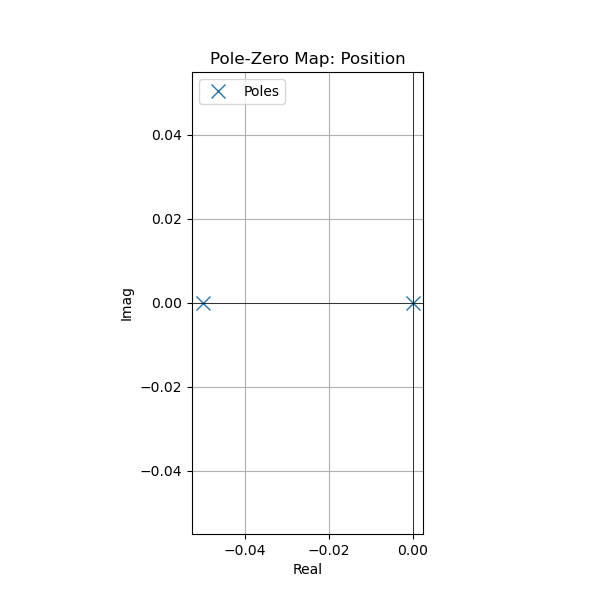
\includegraphics[width=\linewidth]{Figures/car_position_poles.png}
\end{subfigure}
\hfill
\begin{subfigure}[b]{0.48\textwidth}
\centering
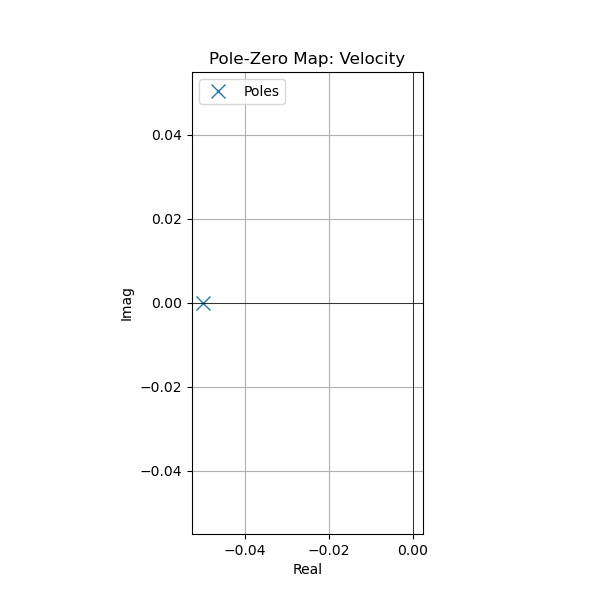
\includegraphics[width=\linewidth]{Figures/car_velocity_poles.png}
\end{subfigure}
\caption{Poles of Car System (Position (left) and Velocity (right))}
\label{f:car_poles}
\end{figure}
Notice that the poles of the position system are located at $s=0$ and $s=-\sigma$ while the pole of the velocity system is located at $s=-\sigma$. The position system has one marginally stable pole and one stable pole while the velocity system has one stable pole. Thus, the position system is marginally stable while the velocity system is stable. Remember if at least one pole is marginally stable and none are unstable the system is considered marginally stable. If all poles are stable the system is considered stable.

\subsubsection{Position of a Mass Spring Damper}

As derived earlier the transfer function for the position of the mass spring damper is given as 
\begin{equation}
    \frac{X(s)}{F(s)}= G(s) = \frac{{\omega_n}^2}{s^2 + 2\zeta \omega_n s + {\omega_n}^2}
\end{equation}
recall also that the time domain solution to this system due to a step function was given as 
\begin{equation}
    x(t) = f_0 \left( 1 - e^{-\zeta \omega_n t} \left( \cos(\omega_d t) + \frac{\zeta}{\sqrt{1-\zeta^2}} \sin(\omega_d t) \right) \right)
\end{equation}
for the underdamped case. Plotted in the time domain the system oscillated and then attained a steady state value. The poles of the system are located at 
\begin{equation}
    s = -\zeta \omega_n \pm j \omega_n \sqrt{1-\zeta^2}
\end{equation}
The real part of the poles is $-\zeta \omega_n$ which is negative for all positive values of $\zeta$ and $\omega_n$. Thus, the system is stable for all positive values of $\zeta$ and $\omega_n$. Examining the system in the laplace domain is much easier than examining the time domain solutions because you can simply look at the poles of the transfer function. It is also beneficial to plot the poles of the system on a real-imaginary plot as shown in Figure \ref{f:mass_spring_damper_poles}.
\begin{figure}[H]
\centering
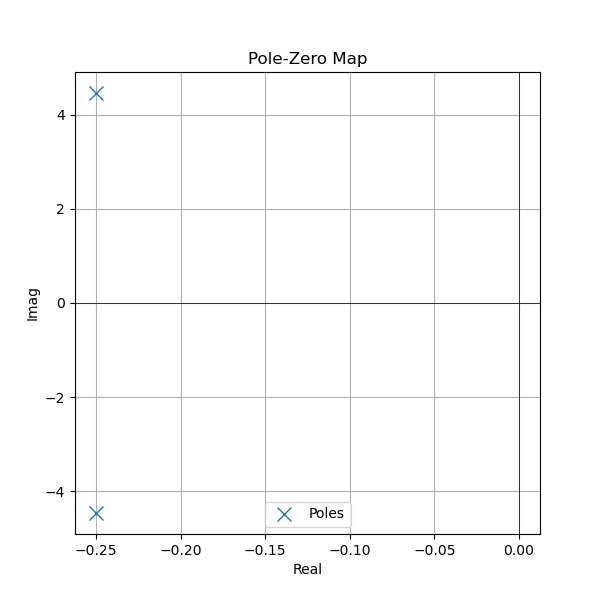
\includegraphics[width=0.6\linewidth]{Figures/mass_spring_damper_poles.png}
\caption{Poles of Mass Spring Damper System}
\label{f:mass_spring_damper_poles}
\end{figure}
Notice that the poles of the mass spring damper system are located in the left half of the complex plane. The real part of the poles is negative and thus the system is stable. The imaginary part of the poles determines the frequency of oscillation while the real part of the poles determines the rate of decay. The further left the poles are located in the complex plane, the faster the system will decay to its steady state value. Thus again the transfer function shows it's usefuleness in determining the stability of a system as well as whether it oscillates or not. In this case the system is stable (left half plane) and oscillatory (imaginary part non-zero).

\subsubsection{Attitude Dynamics of a Satellite or Quadcopter}

\subsubsection{Pitch Dynamics of an Aircraft}

\subsubsection{Pitch Dynamics of a Rocket}

\subsubsection{Angle of an Inverted Pendulum}
